\documentclass[a4wide, 11pt]{article}
\usepackage{a4, fullpage}
\setlength{\parskip}{0.2cm}
\setlength{\parindent}{0cm}
\usepackage[hmargin=2.3cm,vmargin=2.0cm]{geometry}


% This is the preamble section where you can include extra packages etc.

\ifx\pdftexversion\undefined
\usepackage[dvips]{graphicx}
\else
\usepackage[pdftex]{graphicx}
\DeclareGraphicsRule{*}{mps}{*}{}
\fi

\begin{document}

\title{Software Engineering Coursework \\ Design and Implementation of Multiplayer Othello}

\author{Michal Srb and Thomas Rooney}

\date{\today}         % inserts today's date

\maketitle            % generates the title from the data above

\section{Introduction}

The task that we have been given is to design and implement a computer-based version of Othello, that is playable between at least two human players.

To implement this, we have decided to leverage web technologies to build a webpage, that when loaded, provides the player with a UI for a multiplayer lobby, through which the players can challenge one another and play a game of Reversi.

To focus our design efforts, we decided to utilise the Test Driven Development style through the following workflow:
\begin{enumerate}
\item Writing Calling Code
\item Write a shell implementation of the feature, just enough such that it compiles
\item Use Test Driven Development:- writing tests for the feature using the methods defined above; defining the methods such that tests pass \ldots
\item End up with finished, and tested feature
\end{enumerate}

In designing each component, we also attempted to adhere to \texttt{Object Oriented} principles, wherby the number of public methods in each class is minimized to the bare requirement of the features that are inherently necessary to the functionality of the object. This leads to a clean, and simple design.

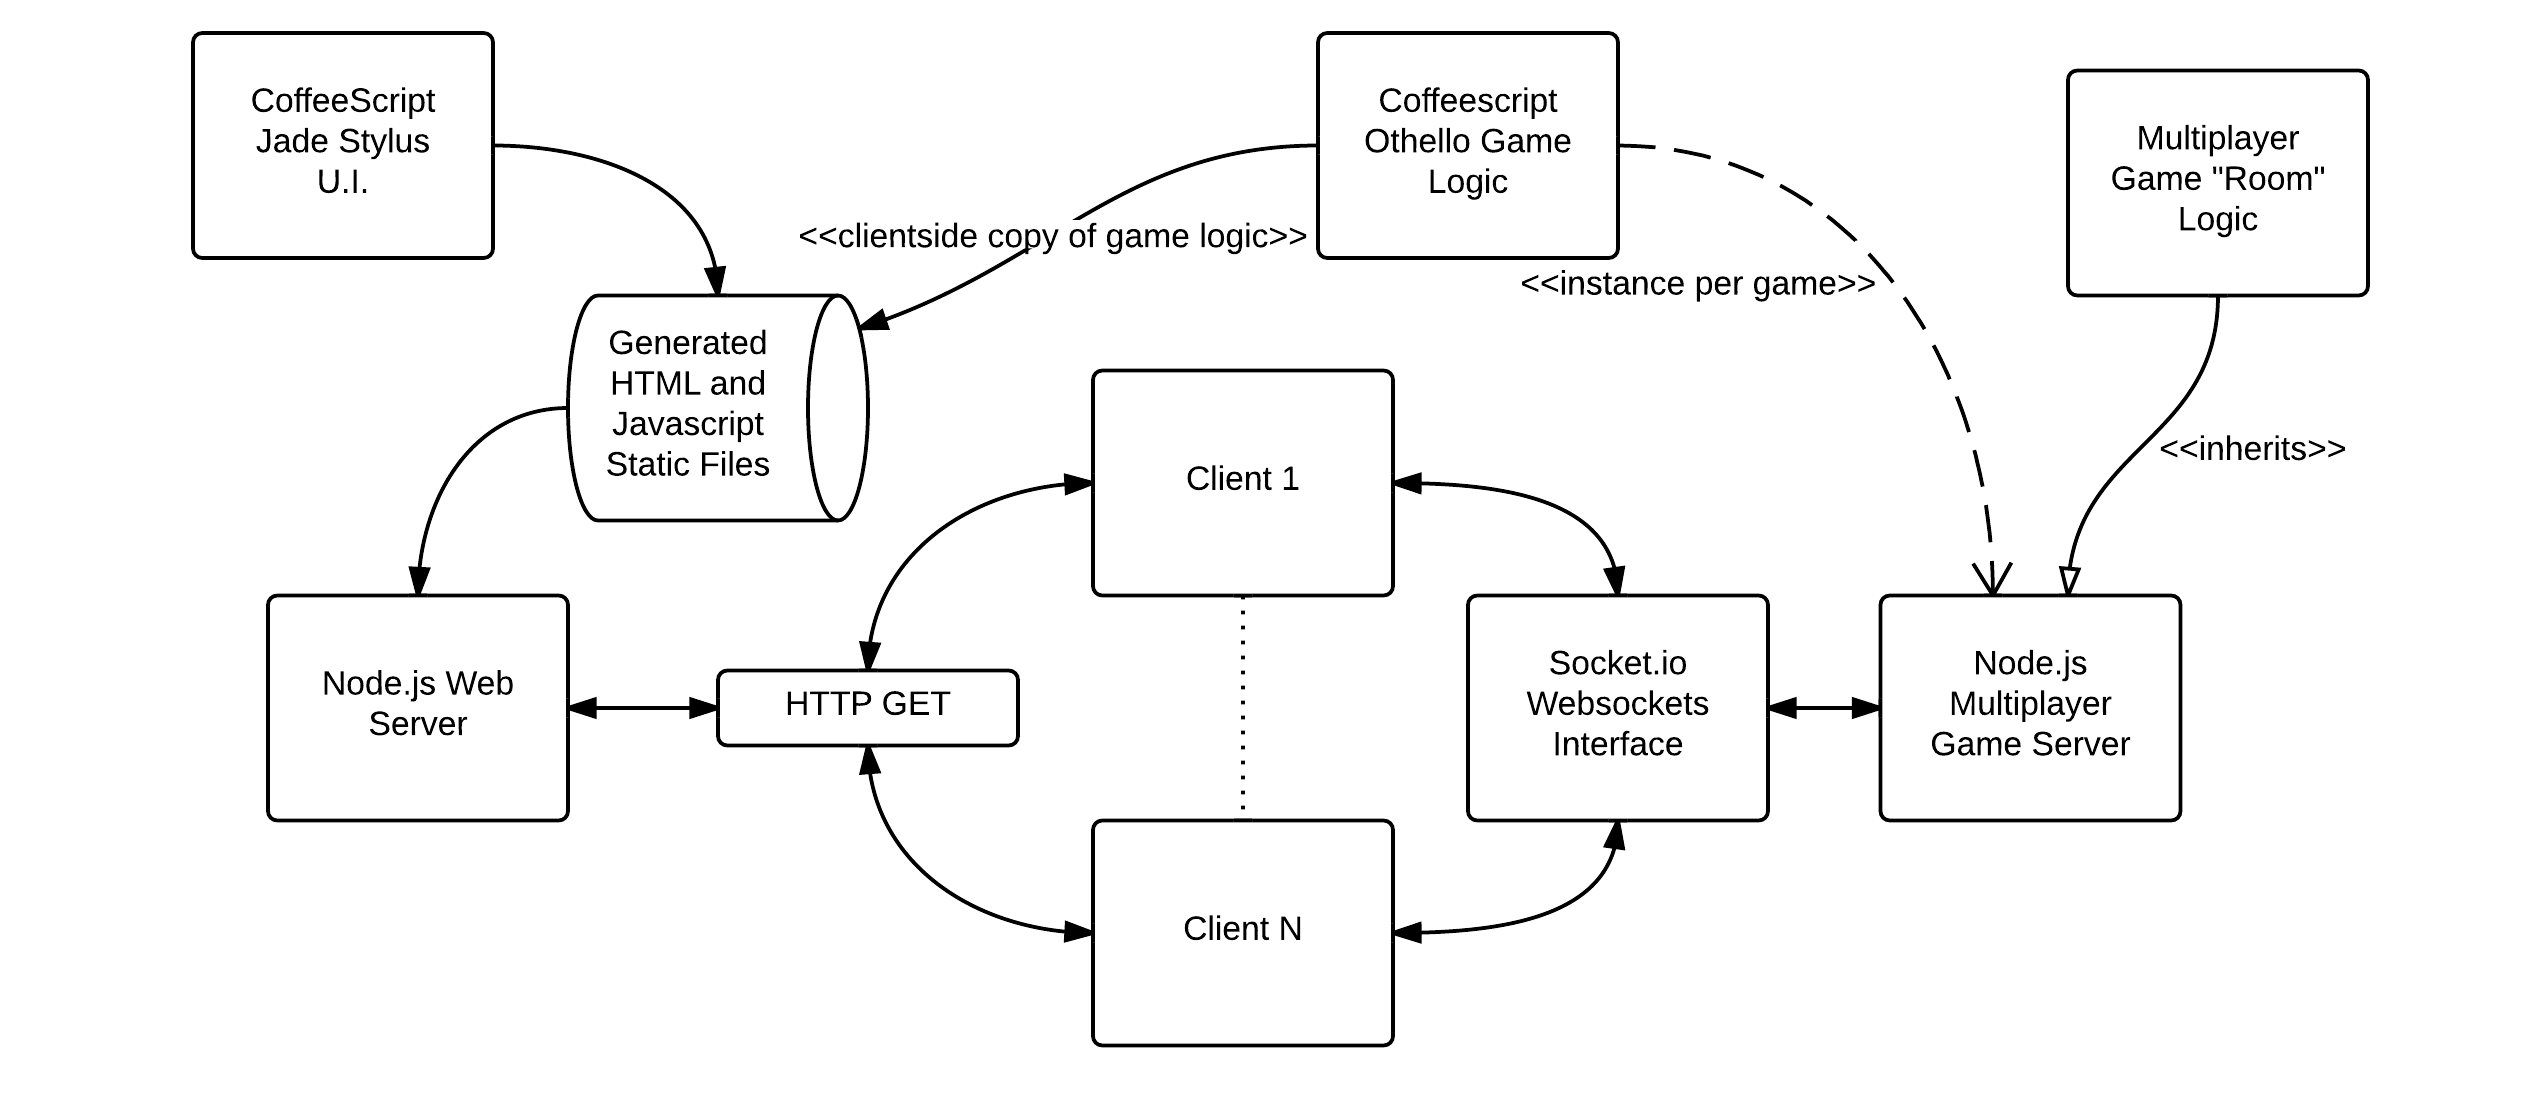
\includegraphics[width=\textwidth]{SoftwareEngineering.png}

\pagebreak

\section{Designing the Othello Game}

\pagebreak
\section{...}
\pagebreak
\section{Designing the User Interface and Networking}
\pagebreak
\section{...}
\pagebreak
\section{Conclusion}
\end{document}
